\documentclass[a4paper]{report}

%====================== PACKAGES ======================

\usepackage[french]{babel}
\usepackage[utf8x]{inputenc}
%pour gérer les positionnement d'images
\usepackage{float}
\usepackage{amsmath}
\usepackage{graphicx}
\usepackage[colorinlistoftodos]{todonotes}
\usepackage{url}
\usepackage[acronym,nomain]{glossaries}
%pour les informations sur un document compilé en PDF et les liens externes / internes
\usepackage{hyperref}
%pour la mise en page des tableaux
\usepackage{array}
\usepackage{tabularx}
%pour utiliser \floatbarrier
%\usepackage{placeins}
%\usepackage{floatrow}
%espacement entre les lignes
\usepackage{setspace}
%modifier la mise en page de l'abstract
\usepackage{abstract}
%police et mise en page (marges) du document
\usepackage[T1]{fontenc}
\usepackage[top=2cm, bottom=2cm, left=2cm, right=2cm]{geometry}
%Pour les galerie d'images
\usepackage{subfig}

\makeglossaries

%====================== INFORMATION ET REGLES ======================

%rajouter les numérotation pour les \paragraphe et \subparagraphe
\setcounter{secnumdepth}{4}
\setcounter{tocdepth}{4}

\hypersetup{							% Information sur le document
pdfauthor = {Nicolas Tanguy,
			Jordan Arzel
		    },			% Auteurs
pdftitle = {Projet de développement MGP321 -
			Développement d'un système de portfolio basé sur un cloud personnel},			% Titre du document
pdfsubject = {Rapport de Projet MGP321},		% Sujet
pdfkeywords = {telecombretagne, cozycloud, cloud,nodejs,angularjs,client-side},	% Mots-clefs
pdfstartview={FitH}}					% ajuste la page à la largueur de l'écran
%pdfcreator = {MikTeX},% Logiciel qui a crée le document
%pdfproducer = {}} % Société avec produit le logiciel

%======================== DEBUT DU DOCUMENT ========================

\begin{document}

%régler l'espacement entre les lignes
\newcommand{\HRule}{\rule{\linewidth}{0.5mm}}

%page de garde
\begin{titlepage}
\begin{center}

% Upper part of the page. The '~' is needed because only works if a paragraph has started.

\includegraphics[width=0.35\textwidth]{./logotb}~\\[1cm]

\textsc{\LARGE Télécom Bretagne}\\[1.5cm]

\textsc{\Large }\\[0.5cm]

% Title
\HRule \\[0.4cm]

{\huge \bfseries Projet de développement MGP321\\
Développement d'un système de portfolio basé sur un cloud personnel \\[0.4cm] }

\HRule \\[1.5cm]

% Author and supervisor
\begin{minipage}{0.4\textwidth}
\begin{flushleft} \large
\emph{Auteur:}\\
Nicolas \textsc{Tanguy}\\
Jordan \textsc{Arzel}\\


\end{flushleft}
\end{minipage}
\begin{minipage}{0.4\textwidth}
\begin{flushright} \large
\emph{Encadrant:} \\
Jean-Marie \textsc{Gilliot}\\

\end{flushright}
\end{minipage}

\vfill


\includegraphics[width=0.55\textwidth]{./cozy}~\\[2cm]

% Bottom of the page
{\large \today}
- Version V0

\end{center}
\end{titlepage}

%page blanche
%\newpage
~
%ne pas numéroter cette page
\thispagestyle{empty}
%\newpage

\renewcommand{\abstractnamefont}{\normalfont\Large\bfseries}
%\renewcommand{\abstracttextfont}{\normalfont\Huge}

\begin{abstract}
\hskip7mm

\begin{spacing}{1.3}


Dans le cadre de la formation \gls{FIP} de Télécom Bretagne, un module de projet est proposé aux élèves. Pendant 63 heures, par binôme, un projet de développement technique est demandé. Dans le cadre de ce projet, nous avons choisi un sujet axé sur le développement web car c'est un domaine qui nous passionne tous les deux. Le titre de ce projet de développement est "Développement d'un système de portfolio basé sur un cloud personnel". L'idée est donc de développer une application sous CozyCloud (cloud personnel) pour pouvoir afficher ses acquis de formation et ses acquis professionnels. Cette application sera développé dans le langage Javascript et devra s'adapter à l'architecture existante de CozyCloud.

Dans ce document, nous présentons plusieurs aspects liés à la gestion de projet. Ce rapport présente donc aussi bien le contexte de l'étude, le cahier des charges, mais aussi la description de la démarche utilisée pour le développement ainsi qu'une description technique. L'aspect planification y est aussi bien évidemment indiqué.


\end{spacing}
\end{abstract}


\tableofcontents

\newacronym{MGP}{MGP}{Module de Gestion de Projets}
\newacronym{Sedela}{Sedela}{Self Data for Enhancing Lifelong learning Autonomy}
\newacronym{FIP}{FIP}{Formation d'Ingenieur par Partenariat}

\printglossaries

\thispagestyle{empty}
\setcounter{page}{0}
%ne pas numéroter le sommaire


%espacement entre les lignes d'un tableau
\renewcommand{\arraystretch}{1.5}

%====================== INCLUSION DES PARTIES ======================

~
\thispagestyle{empty}
%recommencer la numérotation des pages à "1"
\setcounter{page}{0}


\chapter{Présentation du contexte}

Dans cette partie, nous présentons le contexte du projet de l'UV MGP321 ainsi que le contexte de notre projet en lui même.

\section{L'UV MGP321}

Le module projet \gls{MGP}321 est proposé aux élèves {FIP}3A. Pendant 63 heures, chaque binôme d'élèves réalise un projet de développement technique. Ce module permet aux élèves une mise en application pratique d'éléments de cours vus pendant le cursus de formation. C'est de plus une occasion pour les élèves de se confronter à des technologies différentes de leur activité d'entreprise. Les élèves sont libres de choisir dans la liste des projets Télécoms et des projets Info-Réseau. Les élèves d'un binôme peuvent donc être d'options différentes. L'encadrement d'un projet peut être fait par plusieurs enseignants.\\ 

Les objectifs pédagogiques sont multiples, aussi bien techniques que méthodologiques : \\

\begin{itemize}
    \item Exploiter ses connaissances, en les élargissant au besoin, pour répondre à un besoin client

\item Reformuler ce besoin sous forme de cahier des charges fonctionnel
\item Établir et gérer le déroulement du travail en équipe, être réactif, savoir s'adapter aux aléas
\item Utiliser efficacement des outils de travail collaboratif (forge logicielle, outils de planification, ...)
\item Rédiger un rapport de projet qui répond aux attentes des différentes parties
\item Faire une présentation synthétique et critique de ses travaux \\

\end{itemize}

\par
\\ Les livrables suivants concluent le projet : \\
\begin{itemize}
    

\item une réalisation technique avec analyse critique des résultats présentée devant un jury
\item un rapport écrit
\item une soutenance orale
\end{itemize}

\section{Le projet Sedela}

Le projet Sedela "Self Data for Enhancing Lifelong learning Autonomy" est un projet de recherche qui travaille sur le contrôle d'usage partagé de donnée. C'est dans ce contexte que s'inscrit notre projet de MGP321. \\

Dans ce cadre, une application web doit être expérimentée et être testée par des vrais étudiants dans quelques mois. Cet outil prendra la forme d'un portfolio et devra répondre à plusieurs requêtes. La liste des fonctions qui sont attendues à terme sont disponibles dans la partie cahier des charges de ce rapport. Le but du projet est de commencer le développement de cet outil. \\

Un prototype de portfolio avait déjà été réalisé l'année passée par un étudiant de Télécom Bretagne. L'idée initiale pour notre projet de MGP321 était de s'inspirer, voire de repartir de ce prototype pour le compléter pour se mettre en accord avec les nouveaux besoins du client. Ensuite, notre projet sera poursuivi par un autre étudiant de Télécom Bretagne. Il est donc très important de faire en sorte que le projet soit pérenne, notamment en terme d'architecture ou de technologie utilisée afin de faciliter la poursuite de son développement. La première étape de ce projet a donc été de faire une analyse de l'existant, afin de mieux appréhender une éventuelle reprise de celui-ci.






 
\chapter{Cahier des charges fonctionnel}

Dans cette partie, nous présentons le cahier des charges fonctionnel du projet de développement \gls{MGP321}

\section{Présentation d'ensemble du projet}

\subsection{Présentation de l’équipe en charge du projet}

Dans le cadre du projet de développement de troisième année de la formation FIP de l’IMT Atlantique, deux étudiants sont en charge d’une implémentation d’une première version du projet Sedela. Il s’agit de Jordan Arzel et de Nicolas Tanguy. Le projet de FIP de 3ème année a une durée de 3 semaines à temps plein. \\

Un étudiant de troisième année de la formation FIG de l’IMT Atlantique participe aussi, à mi-temps, à la réalisation de ce projet et assurera le développement futur de l’application, après la fin du projet FIP. Il aura pour but de poursuivre l’implémentation du projet et de sa mise en œuvre auprès des futurs étudiants de l’université de Rennes 2.

\subsection{Situation actuelle et problèmes rencontrés}

Actuellement, il n’existe pas d’outil de type Portfolio satisfaisant pour exposer ses compétences dans les universités. \\

De plus, deux principaux problèmes ont été identifiés: \\

\begin{itemize}
    \item de manière générale, la réflexion pédagogique menée en amont de la production et/ou du choix d’un outil est trop souvent insuffisante (voire inexistante) ; ce qui a pour conséquences :
    \item d’avoir un outil rarement adapté aux besoins / services du projet pédagogique
    \item qui est à plus ou moins long terme abandonné (exemples : abandon de Wordpress car trop technique; abandon de Mahara car paramétrage échappant aux équipes pédagogiques (+ absence de communication en réseaux sur les besoins réels de terrain); abandon de Wix (question d’ergonomie) ; limites et contraintes des ENT…)
\end{itemize}


\subsection{Les objectifs du projet }

L’objectif principal du projet est de réaliser un « Portfolio » : un portfolio est un dossier personnel dans lequel les acquis de formation et les acquis de l’expérience d’une personne sont exposés, en vue d’une reconnaissance personnelle ou celle d’un employeur. C’est un « portefeuille » de connaissance. \\

Le but est de créer et d’expérimenter un outil pour l’utilisation et le classement des données personnelles, formatives, ou professionnelles, et ce dans une démarche d’apprentissage tout au long de la vie.	


\subsection{La cible de ce projet}

La cible de l’outil produit sera dans un premier temps les étudiants de l’université de Rennes 2 et de l’UBO dans un but d’expérimentation de l’outil. 
Dans un second temps, l’idée est de proposer cet outil à tous les étudiants et anciens étudiants.


\subsection{Périmètre du projet}

Les pages seront accessibles sur tous types de plateformes (mobiles notamment).


\section{Description graphique et ergonomique}

\subsection{Charte graphique & design:}

Pour la partie privée, nous utiliserons la charte graphique de Cozy Cloud.

Pour la partie publique, nous utiliserons un design moderne (ex : Bootstrap).

\subsection{Maquette}

Voici plusieurs maquettes :

\section{Description fonctionnelle et technique}

\subsection{Description fonctionnelle}

A terme, les fonctions générales du portfolio attendus sont les suivantes :

Fonctions principales : \\

\begin{itemize}
    \item Possibilité de renseigner ses informations personnelles (page privée) : Création de son «profil : Nom, prénoms, adresse, etc. Emploi, formations…
    \item Possibilité de publier son CV (page publique)
    
    \item Possibilité d’avoir un espace où l’on peut déposer des documents

\end{itemize}

Fonctions annexes : \\

\begin{itemize}
    \item Synchronisation des données personnelles : Import des contacts
    \item ¬	Mise à disposition d’un agenda : Import d’agenda
    \item ¬	Ajout d’outils complémentaires :Vidéo, tchat, espaces de travails partagés


\end{itemize}

\subsection{Contraintes techniques}

Nous utiliserons la plateforme de cloud personnelle Cosy Cloud pour développer notre portfolio. Celui-ci sera en fait une application à part entière de notre plateforme Cosy Cloud. Notre application devra donc utiliser le langage JavaScript pour les pages web (plateforme NodeJS), et reposera sur Mongo DB pour la base de données. \\
Les données seront stockées de façon privée sur Cozy Cloud. 


\section{Objectifs du projet en FIP3A (MGP321)}

\subsection{Prestations attendus pour le projet }

Pour le projet FIP 3A, les objectifs sont les suivants :

\begin{itemize}
    \item Réalisation d'une page d'accueil : page comportant, si le profil n'est pas rempli un message d'alerte.
    \item Réalisation d'une page de profil : chaque utilisateur doit être en mesure de renseigner son profil utilisateur, de le modifier. 
    \item Réalisation d'une page de "gestion des stages" : gestion et suivi du stage (ajout et sauvegarde de documents, formulaires de suivi de stage) \\
\end{itemize}

\\Les fonctions attendus lors de ce projet de FIP3A sont réduits compte tenu du fait de la formation à réaliser sur l'outil à utiliser et au temps réduit pour réaliser ce projet.

\chapter{Analyse de l'existant}

L'an passé, un étudiant de la filière FIG, Cédric Patchane, a développé un prototype d'application de Portfolio sur CozyCloud.
Dans cette partie, nous allons faire une analyse de son travail d'un point de vu architecture et de langages utilisés.

\section{Plate-forme de développement utilisée}

\subsection{Présentation de CozyCloud}

CozyCloud est une plateforme de Cloud personnel personnalisable et open-source.  L’outil est entièrement modulaire, et vous offre la possibilité d’installer les fonctionnalités dont vous avez besoin. Il peut s'agir d'applications développées par la communauté ou par vous-même. La différence avec les autres serveurs de Cloud personnel est que Cozy met l'accent sur la collaboration des applications autour des données personnelles de l'utilisateur. Ainsi les applications d'agendas ou de contacts utilisent les mêmes données et sont donc synchronisées. Les applications peuvent être installées depuis la plateforme de développement collaboratif Github ou depuis le catalogue d'application de Cozy ( cf figure 2.2).

\begin{figure}[!ht]
\begin{center}
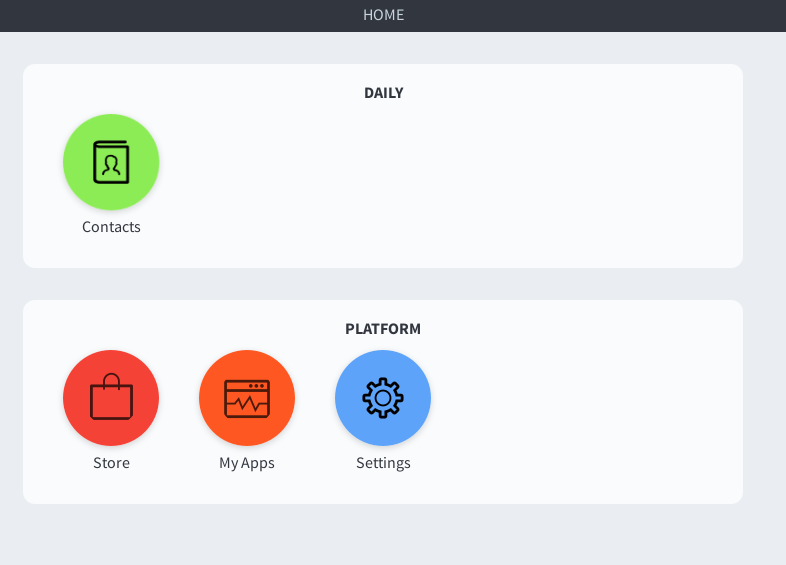
\includegraphics[scale =0.5]{img/cozy_home.png}
\end{center}
\caption{Page home de Cozy Cloud}
\end{figure}

\begin{figure}[!ht]
\begin{center}
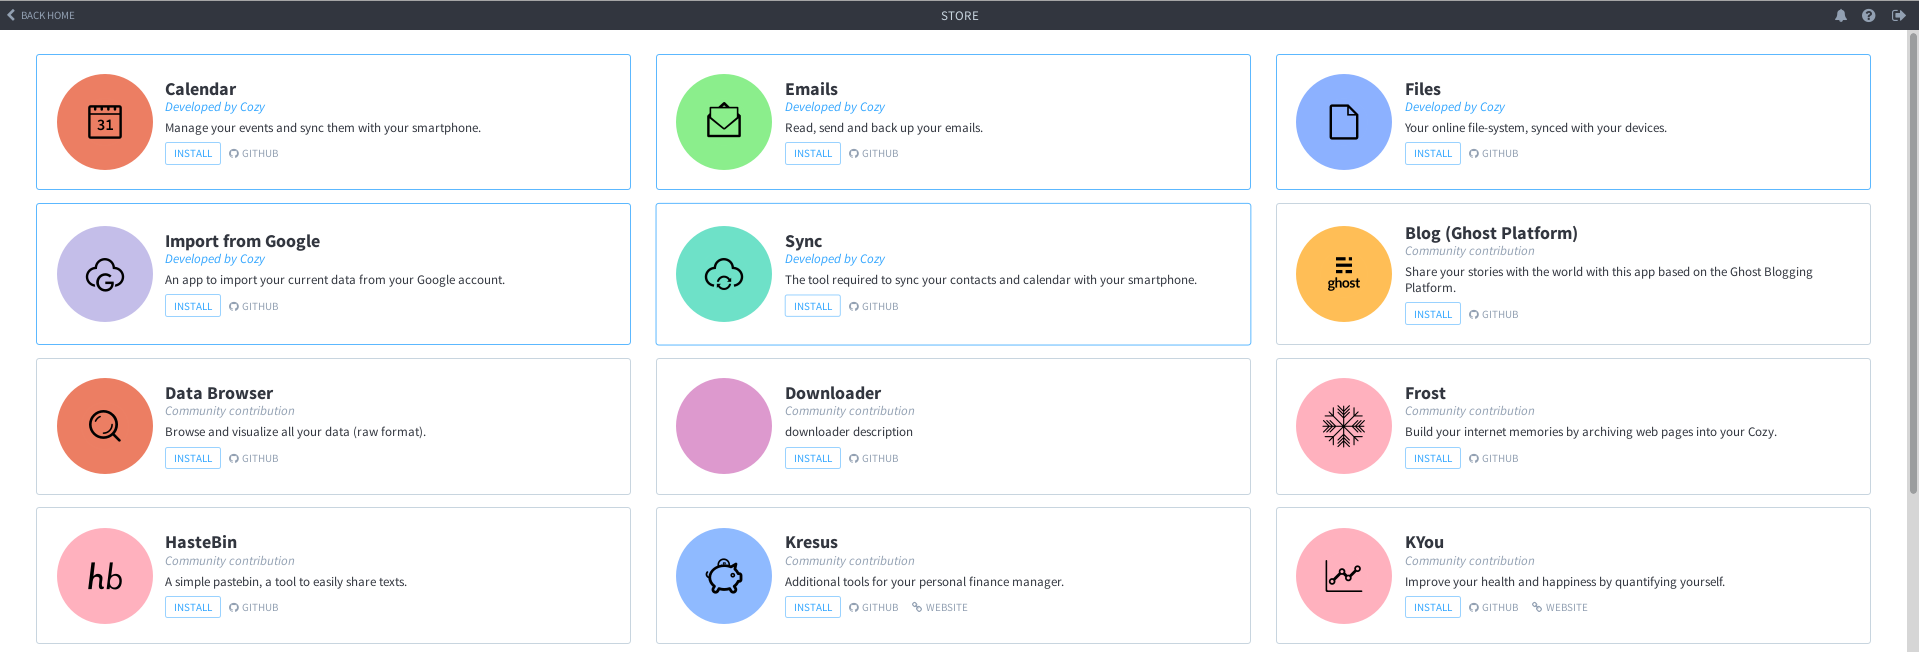
\includegraphics[scale = 0.3]{img/store.png}
\end{center}
\caption{Store de Cozy Cloud}
\end{figure}

\subsection{Architecture et langages utilisés pour le prototype}

Le prototype développé par Cédric Patchane lors de son projet de période 5 se base sur l'architecture de la version 1 de Cozy Cloud. Nous détaillerons ici cette architecture ainsi que le fonctionnement de son application. 

\subsubsection{Environnement de développement}

Pour pouvoir développer des applications pour Cozy, il faut installer un environnement de développement spécifique. En effet, pour pouvoir fonctionner sous CozyCloud, une application nécessite plusieurs outils:\\ 

\textbf{Github :} le premier outil et l'un des plus précieux aux yeux de Cozy est Github. 
Github est un outil de gestion de développement logiciel basé sur le logiciel de version Git. 

Github est l'un des piliers du développement d'applications pour CozyCloud. En effet :

\begin{itemize}
    \item Il favorise la diffusion et le partage de code, et donc de l'open-source.
    \item Mettre son projet sur Github est le seul moyen d'installer une application "maison" sur son Cozy. \\
\end{itemize}

\textbf{Node JS} : Jusqu'à très récemment, le Javascript était uniquement utilisé du côté client. En effet, le navigateur web du visiteur exécutait le Javascript pour effectuer des actions sur la page.
Ceci n'est plus vrai à 100\% désormais. En effet, du code Javascript peut maintenant être exécute du côté serveur. Il est donc désormais possible de générer des pages web directement avec du Javascript. 

Ce serveur NodeJS est donc le second pilier du développement d'applications web pour Cozy cloud. NodeJs permet également de lancer les commandes de développement comme la commande cozy:dev. \\


\textbf{VirtualBox et Vagrant}

VirtualBox est utilisé pour émuler un système d'exploitation complet dans une machine virtuelle. En effet, Cozy est une instance qui tourne sur une machine virtuelle Debian. Celle-ci permet de faire tourner tous les services, comme la base de donnée, etc.

Vagrant est un CLI (Commande Line Interface) qui permet d'interragir avec des commandes avec VirtualBox. Cela permet un développement plus rapide et plus facile. \\

\subsubsection{Présentation de l'architecture de Cozycloud}

La figure~\ref{fig:figArchi} présente la structure de l'architecture de CozyCloud. 

\begin{figure}[!ht]
\begin{center}
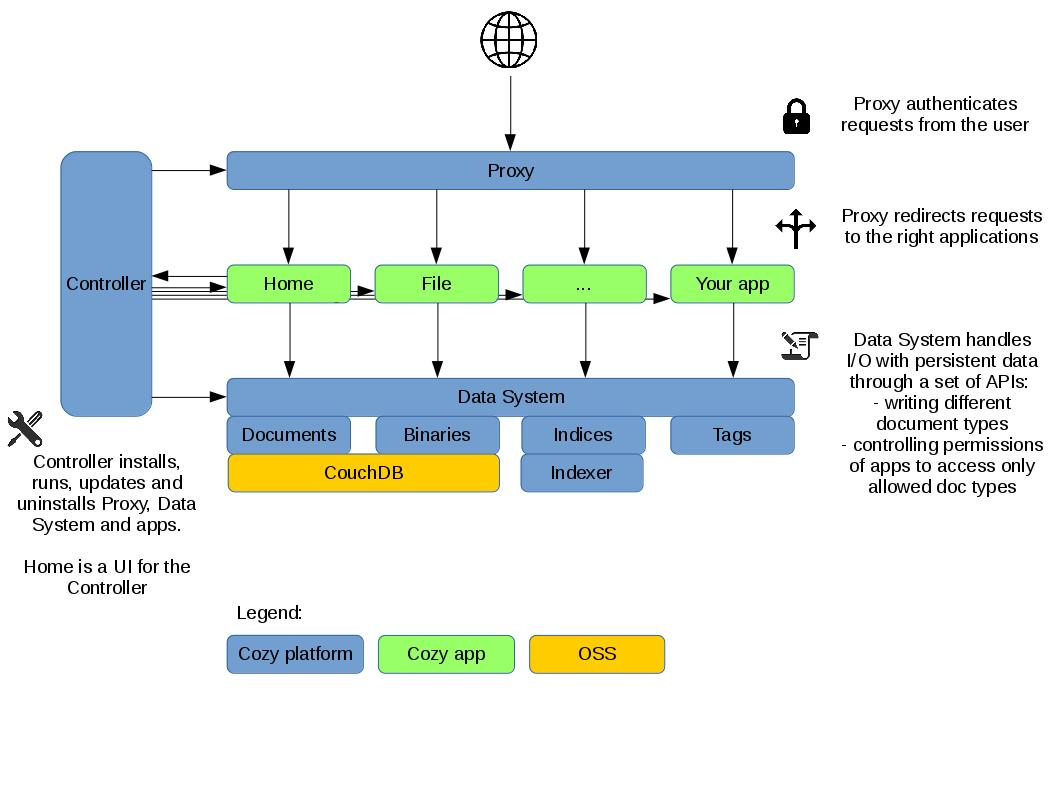
\includegraphics[scale = 0.3]{img/cozy-architecture.jpg}
\end{center}
\caption{Présentation de l'architecture de CozyCloud}
\label{fig:figArchi} 
\end{figure}

\newpage

Cozy est donc constitué de trois composants principaux : \\

\begin{itemize}
    \item La couche data (data-system) : la couche data est au coeur du de l'architecture de cozy. C'est donc la partie centrale où toutes les données sont sécurisées et stockées. La couche data est en fait une API qui consiste à gérer : la database (CouchDB), lieu où sont stockés toutes les données de Cozy. Comme CouchDB est une database de type NOSQL, les données ne sont pas stockées dans des tables, mais sous forme de document (doctypes). Chaques documents sont de types différents et peuvent contenir n'importe quel format de donnée. De plus, avec Cozy, chaque application possède des droits d'accès spécifiques sur ces données, et donc les applications ne sont pas autorisés à accéder à n'importe quelles données de la base. \\

    \item Le Paas (Platform as a service) : c'est l'environnement d'execution des applications. Cela consiste en fait principalement à un contrôleur qui va installer, exécuter, et mettre à jour les applications de Cozy. 
    
    \item L'interface Plateforme : elle consiste en un home et un proxy (répertoire Github). Le home est l'interface qui va permettre au contrôleur de manager les applications dans cozy. Enfin, le proxy va permettre à l'utilisateur d'interagir avec les données. En effet, le proxy va gérer l'authentification et les autorisations d'accès dans Cozy. Ce dernier gère également le "routing", c'est à dire l'envoi de la bonne requête à la bonne application
    
    
\end{itemize}

\subsubsection{Fonctionnalités de l'application}

L'application développées par Cédric permet de réaliser son propre portfolio dans le cloud personnel Cozy. Cette application dispose de quatre vues :

\begin{itemize}
    \item\textbf{Mon profil} : cette vue permet de renseigner les informations du profil utilisateur (nom,prénom...) comme on peut le voir en figure\ref{fig:vueProfil}. L'utilisateur peut choisir d'afficher ou non les informations renseignées sur son portfolio public. 
    \item \textbf{Vue publique du portfolio} : il s'agit de la vue de l'utilisateur générée en fonction des choix d'affichage des documents effectués par l'utilisateur. 
    \item \textbf{Mes choix} : cette vue regroupe tous les documents de l'utilisateur qui peut les modifier ou les supprimer. Il peut également faire le choix de les afficher ou non dans la vue publique de son portfolio. Il est possible d'ajouter des documents directement depuis cette page. 
     \item \textbf{Paramètres} : C'est ici que l'on peut configurer les comptes DoyouBuzz et OpenBadges (cf figure\ref{fig:vueProfil}.    
\end{itemize}

DoYouBuzz est une palteforme de création de CV en ligne. L'application portfolio permet de rapatrier son CV dans son cloud personnel Cozy et ce, via un API. OpenBadges est une représentation de la réussite sous forme de badges. Elle permet de visualiser de façon détaillée l'apprentissage tout au long de la vie d'une personne. Les badges sont récupérés  grâce à l'e-mail associé au compte dans la partie publique d'OpenBadges. Une vue de cette page est disponible en figure~\ref{fig:vueConfigCompte}. 


\begin{figure}[!ht]
\begin{center}
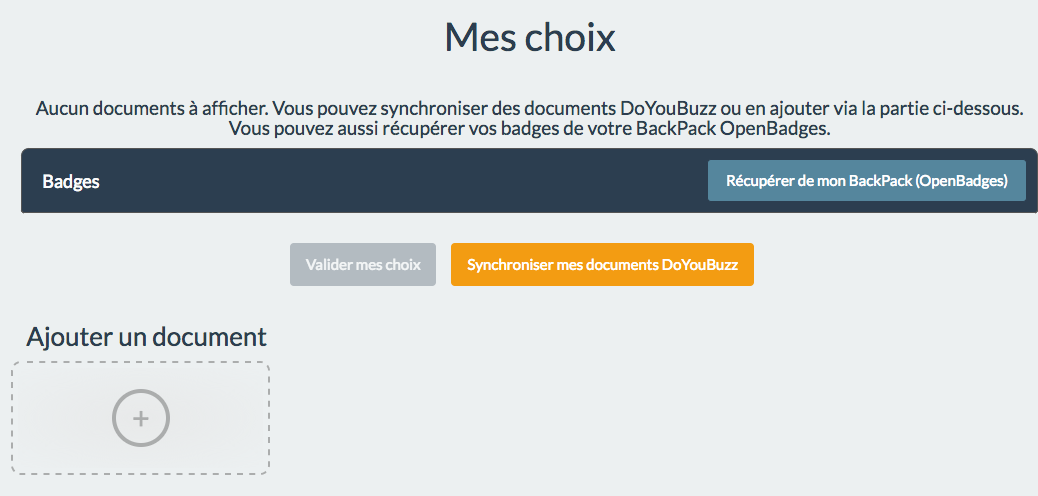
\includegraphics[scale = 0.3]{img/ajout-badges.png}
\end{center}
\caption{Vue de la page ajout des badges}
\label{fig:vueBadge} 
\end{figure}


\begin{figure}[!ht]
\begin{center}
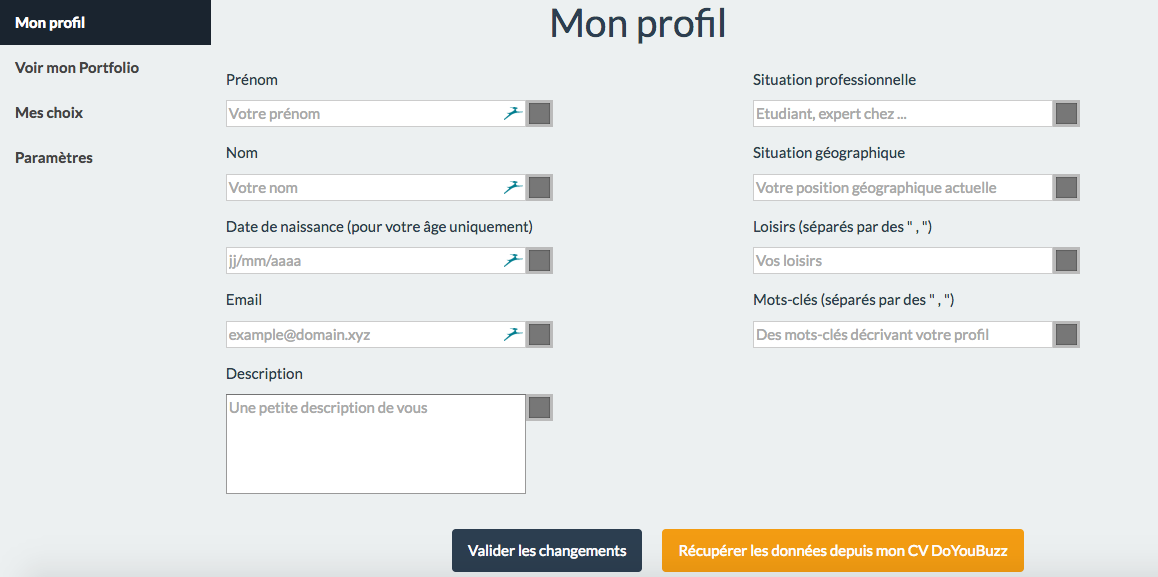
\includegraphics[scale = 0.3]{img/mon-profil.png}
\end{center}
\caption{Vue de la page mon profil}
\label{fig:vueProfil} 
\end{figure}

\begin{figure}[!ht]
\begin{center}
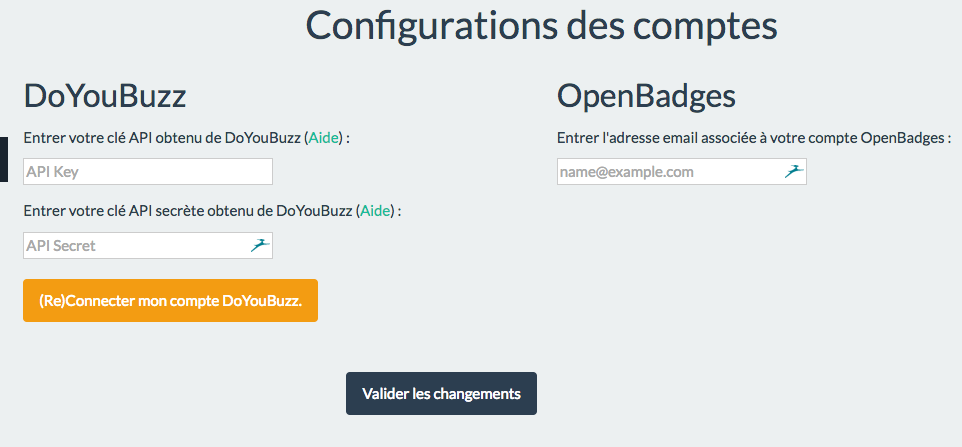
\includegraphics[scale = 0.3]{img/config-comptes.png}
\end{center}
\caption{Vue de la page configuration des comptes}
\label{fig:vueConfigCompte} 
\end{figure}

\section{Choix de repartir d'une nouvelle base}

Après des discussions avec les différents membres présents ou passés du projet (Florian Coste et Cédric Patchane notamment), il nous est apparu nécessaire de repartir sur une nouvelle base. En effet, l'architecture de Cozy est en pleine évolution et la v3 devrait être disponible dans les prochains mois (annoncée pour mars 2017). L'application développée par Cédric correspond à une architecture type v1 et est décomposée en une partie cliente et une partie serveur. Cette dernière est difficilement maintenable par le développeur d'applications au gré des évolutions de librairies tierces par exemple. Le choix de l'équipe de Cozy fut de pousser le développement d'applications de type "clientsideapps" ou la partie serveur n'est plus gérée par le développeur mais par Cozy. Nous avons fait le choix de développé de cette manière pour rendre compatible notre application avec la version 2. A terme, nous nous sommes assurés par le biais d'échanges avec l'équipe Cozy (Cédric mais aussi le channel IRC), que l'application serait facilement migrable vers la version 3. 

Pour conclure cette partie, on peut donc dire que la phase d'analyse nous a permis de comprendre l'existant mais aussi de se rendre compte qu'il fallait en modifier l'architecture. Nous verrons plus en détail par la suite, les choix que nous avons effectués. 




\chapter{Développement technique}



\section{Choix techniques et architecture mise en oeuvre}

Nous allons voir dans cette partie les choix que nous avons effectués au niveau technique et les fonctionnalités que nous avons implémentées. 
\subsection{Une application "clientside"}

L'architecture version 2 de Cozy Cloud permet le développement d'applications en ne se focalisant que sur le développement de la partie cliente (frontend). Cozy propose une API pour accéder et gérer les données de l'utilisateur. De plus l'authentification est également gérée par Cozy, ce qui permet de ne se concentrer que sur les fonctionnalités que l'on souhaite mettre en oeuvre. Cela permet également de choisir son framework favori pour développer.  

\newpage{}

\subsection{Un framework frontend : AngularJS}

Nous avons choisi de développer en utilisant le framework AngularJS de Google. Ce choix s'explique par deux raisons principales : 

\begin{itemize}
\item Premièrement, il s'agit du framework sur lequel nous possédions le plus de connaissances;
\item Deuxièmement, le tutoriel disponible propose une partie dédiée à AngularJS;
\end{itemize}

Ainsi un squelette d'application cliente était disponible de le répertoire Github de Cozy. Ce fut un point de départ intéressant pour nous. L'application se décompose en trois partie architecturées en MVC (Model-View-Controller). Ici le modèle est fourni par Cozy pour les fonctionnalités de CRUD (Create Read Update Delete). Les vues sont organisées de manières à ce quelles soit chargées par le biais d'un menu unique. Elles vont affichés le contenu (formulaires de saisie, documents dans la base). En ce qui concerne les contrôleurs, ce sont eux qui vont faire le lien entre la vue (et la saisie de l'utilisateur par exemple) et l'insertion ou lecture dans la base par le biais des fonctions de CRUD.  



\newpage


\section{Fonctionnalités développées}

\subsection{Les fonctionnalités}
\subsection{Le modèle de données}
\subsection{Les améliorations possibles et les fonctionnalités à développer}

\chapter{Démarche utilisée}

Ce chapitre présente la démarche utilisée aussi bien pour la gestion de notre projet que notre façon d'aborder le développement technique de la solution réalisée.

\section{Gestion de projet}

Au cours de ces trois semaines, afin d'atteindre l'objectif fixé, il était essentiel d'avoir des bonnes méthodes de gestion de projet. Dans cette partie, nous expliquons les méthodes mises en oeuvre pour dans le cadre de cette gestion de projet.

\subsection{Planification}

Une des premières étape de la gestion de projet a été de planifier ces trois semaines. Cette étape permet de déterminer et surtout d'ordonnancer les tâches à réaliser pendant le projet. Elle permet également d'estimer leurs charges.\\

Pour mener à bien cette étape de réalisation, nous avons choisi de mettre en oeuvre un Gantt. Ce Gantt permet :

\begin{itemize}
    \item Déterminer si les objectifs sont réalisés ou dépassés
    \item Suivre et communiquer l’avancement du projet
    \item Affecter les ressources aux tâches

\end{itemize}

Le Gantt prévisionnel est disponible sur la figure~\ref{fig:gantt_prev}

\begin{figure}[!ht]
\begin{center}
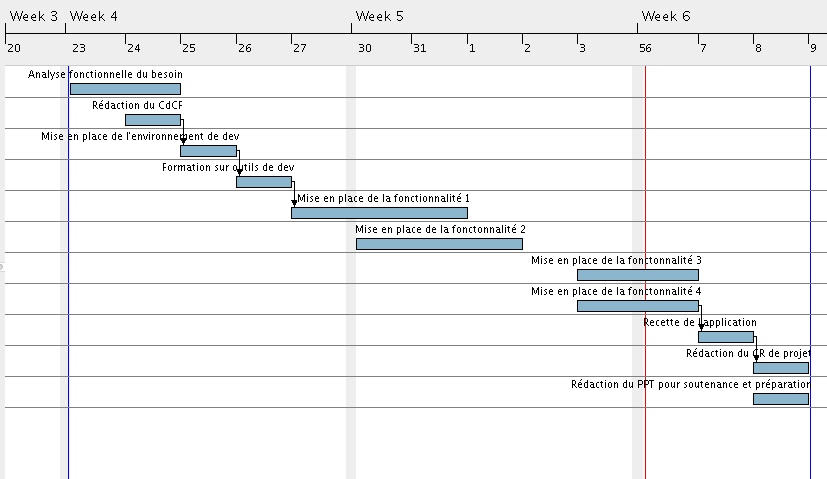
\includegraphics[scale = 0.3]{img/gantt-prev.png}
\end{center}
\caption{Gantt Prévisionnel}
\label{fig:gantt_prev} 
\end{figure}

Le Gantt réel est disponible sur la figure ..

\section{Gestion du développement technique}

Dans cette partie, nous expliquons la façon dont nous avons procédé pour gérer le développement technique de l'application.

\subsection{Installation des outils de développement}

La première partie a été l'installation des nouveaux composants nécessaires aux développement d'une application sur l'environnement de CozyCloud. Ces éléments sont ceux cités dans la partie 3.1.2.1.


\subsection{Formation sur l'outil CozyCloud}

C'est une des parties qui nous a pris le plus de temps. En effet, nous ne connaissions par du tout l'environnement de développement, et nous avons fait face à un manque accru de documentation.

Nous avons donc sollicité les développeurs de chez Cozy, directement sur un tchat mis à disposition (IRC channel #cozycloud). Cela nous a permis d'en apprendre davantage sur la plateforme, mais cela nous a également permis, une fois le développement commencé, d'aider à la résolution de nos divers problèmes.

\subsection{Développement des fonctionnalités}

Pour le développement des fonctionnalités, nous nous sommes appuyés sur plusieurs API disponibles. Ainsi, nous avons pu utiliser l'API cozybrowser-sdk. Il a donc fallu par commencer par lire les documentations. \\

Aussi, nous nous sommes aidés d'un tuto "Make a client side-app..." disponible sur le site de cozy-cloud. Il nous a permis de prendre nos repères sur le développement d'application client-side et de débuter la programmation de notre application My Portfolio.

\chapter{Bilan \& résultats}

Dans ce chapitre, nous allons faire un bilan d'un point de vue technique et organisationnel.

\section{Bilan technique}

\subsection{Avancement du projet}

Concernant l'avancement du projet, nous sommes très déçus de ne pas avoir pu réaliser toutes les fonctions initialement prévues. Nous n'avons souvent pas réussis à trouver des réponses à nos questions techniques par le manque de documentation présentes sur le web. De plus, comme c'est une architecture et des façons de développer différentes (client-side app), nous avons mis beaucoup de temps à tenter de comprendre comment développer telle ou telle fonction. \\

Peut être que nous avons été trop ambitieux sur le nombre de fonction à réaliser, mais nous n'aurions pas pu prévoir le changement de programme (nous devions repartir de zéro) qui est arrivé lors de la deuxième semaine de notre projet.

\subsection{Apprentissage technique}

D'un point de vue technique, nous avons pu acquérir de nombreuses connaissances. En effet, avant le projet, seul Jordan connaissait le NodeJS et AngularJs. Maintenant, nous sommes à l'aise sur ces technologies. De plus, nous avons appris le concept de création d'une app client-side, ce qui est intéressant pour nous pour la suite de notre cursus.

\section{Bilan organisationnel du projet}

\subsection{Répartition des tâches}

Au cours de ce projet, nous avons beaucoup travaillé ensemble à la compréhension de l'architecture de l'application réalisée par Cédric Patchane l'an dernier. Cela nous a permis de nous expliquer mutuellement les choses que l'on comprenaient et celles que l'on ne comprenaient pas. \\

Puis, quand nous avons commencé à développer, comme nous avons fait face à de gros soucis technique avec Cozy, nous nous sommes beaucoup aidés mutuellement. 

Cependant, lors de la réalisation de la partie graphique, par exemple, nous nous sommes séparés les tâches : chacun à réalisé plusieurs des pages proposées.





%Ne pas numéroter cette partie
\part*{Annexes}
%Rajouter la ligne "Annexes" dans le sommaire
\addcontentsline{toc}{part}{Annexes}


\listoffigures
%récupérer les citation avec "/footnotemark"
\nocite{*}

%choix du style de la biblio
\bibliographystyle{plain}
%inclusion de la biblio
\bibliography{bibliographie.bib}
%voir wiki pour plus d'information sur la syntaxe des entrées d'une bibliographie

\end{document}